\documentclass[11 pt]{article}

\usepackage{amsfonts}
\usepackage{amsmath}
\usepackage{fancyhdr}
\usepackage[left=2cm,right=2cm,top=2cm,bottom=2cm]{geometry}
\usepackage{graphicx}
\usepackage[hidelinks]{hyperref}
\usepackage{listings}
\usepackage{subfig}
\usepackage{xcolor}
\usepackage{comment}

\pagestyle{fancy}
\fancyhf{}
\lhead{Fundamentals of Simulation Methods}
\chead{Exercise 07}
\rhead{J. Edelmann, V. Mader}
\setlength{\headheight}{15pt}

\newcommand{\pder}[2]{\frac{\partial #1}{\partial #2}} % total derivative
\newcommand{\tder}[2]{\frac{\dd #1}{\dd #2}} % partial derivative
\newcommand{\dd}{\mathrm{d}}
\newcommand{\red}[1]{\textcolor{red}{#1}} 
\newcommand{\blue}[1]{\textcolor{blue}{#1}} 
\newcommand{\green}[1]{\textcolor{green}{#1}} 

\definecolor{commentsColor}{rgb}{0.497495, 0.497587, 0.497464}
\definecolor{keywordsColor}{rgb}{0.000000, 0.000000, 0.635294}
\definecolor{stringColor}{rgb}{0.558215, 0.000000, 0.135316}
% \lstnewenvironment{code}[2][]{%
\lstset{ %
    backgroundcolor=\color{white},   % choose the background color; you must add \usepackage{color} or \usepackage{xcolor}
    basicstyle=\footnotesize,        % the size of the fonts that are used for the code
    breakatwhitespace=false,         % sets if automatic breaks should only happen at whitespace
    breaklines=true,                 % sets automatic line breaking
    % captionpos=b,                    % sets the caption-position to bottom
    commentstyle=\color{commentsColor}\textit,    % comment style
    deletekeywords={...},            % if you want to delete keywords from the given language
    escapeinside={\%*}{*)},          % if you want to add LaTeX within your code
    extendedchars=true,              % lets you use non-ASCII characters; for 8-bits encodings only, does not work with UTF-8
    frame=tb,	                   	   % adds a frame around the code
    keepspaces=true,                 % keeps spaces in text, useful for keeping indentation of code (possibly needs columns=flexible)
    keywordstyle=\color{keywordsColor}\bfseries,       % keyword style
    language=Python,                 % the language of the code (can be overrided per snippet)
    otherkeywords={*,...},           % if you want to add more keywords to the set
    numbers=left,                    % where to put the line-numbers; possible values are (none, left, right)
    numbersep=5pt,                   % how far the line-numbers are from the code
    numberstyle=\tiny\color{commentsColor}, % the style that is used for the line-numbers
    rulecolor=\color{black},         % if not set, the frame-color may be changed on line-breaks within not-black text (e.g. comments (green here))
    showspaces=false,                % show spaces everywhere adding particular underscores; it overrides 'showstringspaces'
    showstringspaces=false,          % underline spaces within strings only
    showtabs=false,                  % show tabs within strings adding particular underscores
    stepnumber=1,                    % the step between two line-numbers. If it's 1, each line will be numbered
    stringstyle=\color{stringColor}, % string literal style
    % tabsize=2,	                   % sets default tabsize to 2 spaces
    % title=#2,                  % show the filename of files included with \lstinputlisting; also try caption instead of title
    columns=fixed                    % Using fixed column width (for e.g. nice alignment)
}%
% }{}


\begin{document}

    \section{Heat diffusion problem \textit{(10 points)}}
    Tree algorithms can approximately calculate the forces in an 
$N$-body system by means of a hierarchical multipole expansion. 
This reduces the computational cost to something of order 
$O(N \ln N)$. On the download page of the lecture, a simple 
skeleton tree code can be downloaded (a C-version as well as a 
Python-version are provided). Note that this implementation uses 
only monopole order and is not optimized for speed or memory 
consumption. You can use this template for this exercise, 
either directly or translated to another language, or if you 
wish, you may also write your own tree code from scratch using 
the template as an example (it’s fun to do! ;-) ). \\
\\
Consider $N$ particles of total mass $M_{\textnormal{tot}}=1$ 
placed randomly into a cubical box of unit side length. For 
definiteness, we assume all particles have the same mass, and 
we adopt $G=1$. Assume that the gravitational potential of 
individual particles is Plummer-softened with a gravitational 
softening length $\varepsilon=0.001$, 
i.e. we adopt the potential
\begin{equation}
    \Phi(\vec r)=-\frac{m}{\sqrt{\vec r^2+\epsilon^2}}
\end{equation}
for a single particle of mass $m$.
Calculate the gravitational forces for all $N$ particles with an 
oct-tree and determine the typical force accuracy and 
calculational time in comparison with direct summation, both as 
a function of $N$ and of the opening angle parameter $\Theta^*$. 
To this end, carry out the following steps:


\paragraph{a) The idea of this exercise is that you use one of 
    the two templates provided (tree.c or tree.py \& call 
    tree.py). But if you like a challenge, you are encouraged 
    to write your own version! As a reference, there is pseudo 
    code provided at the end of the sheet.
} \ \\
    \\
    We chose to work with the template code (see below).


\newpage
\paragraph{b)
    The provided code template is incomplete, so start by filling 
    in the missing pieces. In particular, you need to add the 
    computation of the centers of mass and total masses of tree 
    nodes from their subnodes, as well as the partial force 
    calculation from a tree node that is used in the tree walk. 
    Also, please add a calculation of the exact forces by 
    direct summation. When you are done, verify that the force 
    approximation delivered by the tree code is roughly correct 
    by adding suitable output to the code.
} \ \\
    \\
    Computation of the centers of mass \& total masses of tree nodes: \\
    \\
    tree.py
    \lstinputlisting[firstline=98, lastline=123]{../code/ex8_tree/python/tree.py} \ \\
    \newpage \noindent
    Force calculation: \\
    \\
    tree.py
    \lstinputlisting[firstline=125, lastline=156]{../code/ex8_tree/python/tree.py} \ \\
    \\
    Calculation of exact forces: \\
    \\
    call\_tree.py
    \lstinputlisting[firstline=86, lastline=101]{../code/ex8_tree/python/call_tree.py}

\newpage
\paragraph{c)
    To allow a more quantitative analysis, add an automatic 
    measurement of the average force error after all forces 
    have been calculated by the tree and direct summation.
} \ \\ 
    \\
    To this end, consider the relative force error
    \begin{equation}
        \eta
        =\frac{\vec{a}_\textnormal{tree}-
        \vec{a}_\textnormal{direct}}{\vec{a}_\textnormal{direct}}
    \end{equation}
    for each particle, and determine a simple arithmetic average 
    $\langle\eta\rangle$ of the mean relative force error. Also, 
    add diagnostic code that tells you the average number of 
    particle-node interactions per particle, i.e. how many nodes 
    the multipole expansion on average involves. \ \\
    \\
    Our implementation can be seen below: \\
    \\
    call\_tree.py
    \lstinputlisting[firstline=103, lastline=108]{../code/ex8_tree/python/call_tree.py}


\newpage
\paragraph{d) Make a little grid of calculations for 
    $N=5000, 10000, 20000$ and $40000$, and opening angles 
    $\theta^*=0.2$, $0.4$ and $0.8$. In each case, measure the 
    calculation time for the tree-based force calculation and 
    for direction summation, as well as $\langle\eta\rangle$ 
    and the mean number of terms the tree code used per particle. 
    Report the results in a table.
} \ \\
    \\
    % NOTE: For direct summation with $N=40000$ particles the 
    % calculation could take very long; you can extrapolate from 
    % smaller $N$ cases since we know it scales as $N^2$.
    % Especially Python users might need to run smaller resolution 
    % problems, e.g. divide the number by ten (however, you should 
    % still have at least four different $N$ to be able to 
    % extrapolate). \\
    % \\
    We used Python, therefore we chose to test the algorithm on 
    $N=$ 2500, 5000, 10000 and 20000.
    \begin{table}[h!]
        \begin{center}
        \caption{$t_\textnormal{tree}$ (top) and $t_{N^2}$ (bottom) in seconds}
        \begin{tabular}{c | c | c | c}
            $N$ \textbackslash\ $\theta^*$ & 0.2  & 0.4  & 0.8 \\
            \hline
            2500  & 92   & 25   & 5    \\
                  & 50   & 47   & 47   \\
            \hline
            5000  & 234  & 55   & 11   \\
                  & 168  & 188  & 192  \\
            \hline
            10000 & 755  & 198  & 29   \\
                  & 1574 & 1455 & 1467 \\
            \hline
            20000 & 2666 & 598  & 214  \\
                  & 3888 & 4666 & 4915 \\
        \end{tabular}
        \end{center}
    \end{table} 
    \begin{table}[h!]
        \begin{center}
        \caption{mean number of interactions}
        \begin{tabular}{c | c | c | c}
            $N$ \textbackslash\ $\theta^*$ & 0.2  & 0.4  & 0.8 \\
            \hline
            2500  & 3444 & 824  & 180 \\
            \hline
            5000  & 4020 & 981  & 202 \\
            \hline
            10000 & 5141 & 1155 & 226 \\
            \hline
            20000 & 6220 & 1314 & 248 \\
        \end{tabular}
        \end{center}
    \end{table} 
    For small angles and particle numbers 
    ($\theta^*=0.2$, $N=2500,5000$) the execution time 
    of the direct method is less than that of the tree 
    method. For $\theta^*=0.2$ and $N=2500$,
    the same holds for the mean number of interactions.
    It is interesting to see that the mean number of 
    interactions can surpass the number of particles 
    in the system. The reason for that is that for 
    small angles it can happen that a cell with only a 
    single particle in it is divided again. For large 
    angles and particle numbers, the opposite is true, 
    and the tree method outperforms the direct method.  \\
    \\
    The execution time seems to depend much more 
    strongly on the angle $\theta^*$ than it does on 
    the particle number $N$. 
    \begin{table}[h!]
        \begin{center}
            \caption{relative error $\langle\eta\rangle$}
            \begin{tabular}{c | c | c | c}
                $N$ \textbackslash\ $\theta^*$ & 0.2 & 0.4 & 0.8 \\
                \hline
                2500  & $(0.18\pm0.05)\%$ & $(0.96\pm0.12)\%$ & $(29.44\pm31.82)\%$ \\
                \hline
                5000  & $(0.13\pm0.02)\%$ & $(1.10\pm0.22)\%$ & $(8.18\pm1.96)\%$ \\
                \hline
                1000  & $(0.24\pm0.12)\%$ & $(1.05\pm0.20)\%$ & $(8.89\pm2.79)\%$ \\
                \hline
                20000 & $(0.26\pm0.14)\%$ & $(1.01\pm0.27)\%$ & $(8.66\pm5.71)\%$ \\
            \end{tabular}
        \end{center}
    \end{table} \ \\ 
    The relative error $\langle\eta\rangle$ seems to 
    grow with the angle $\theta^*$. There is not 
    really a trend to be seen for the relative error
    as a function of $N$. There is one notable
    outlier for $\theta^*=0.8$ and $N=2500$.

% \newpage
\paragraph{e)
    Using the previous results, make a plot of the execution 
    time of the force calculation with the tree as a function of 
    $N$ (for the $\theta_c=0.4$ case). Use logarithmic axes and 
    fit a regression line (in the log) to the 4 data points you 
    obtained. Also include the results for direct summation. 
    Estimate the time needed for $10^{10}$ particles for both 
    methods.
} \ \\
    \begin{figure}[h!]
        \centering
        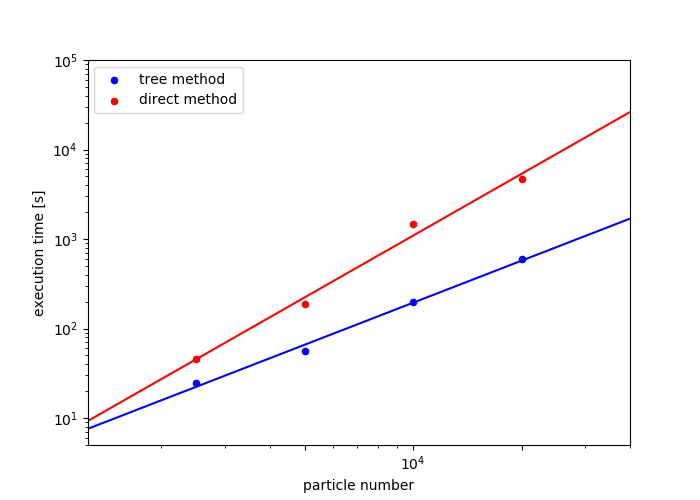
\includegraphics[width=\textwidth]{../plot/runtimes.png}
        \caption{execution time vs. particle number}
    \end{figure} \ \\ 
    For the tree method, we calculated the exponent,
    which is approximately 1.6, while the exponent for 
    the direct method is about 2.3. For $N=10^{10}$, 
    we extrapolate that the tree algorithm would take 
    14 thousand years, while the direct algorithm 
    would take 2 billion years.



    \newpage

    \section{1D multigrid method \textit{(8 points)}}
    In order to simulate the Riemann problem for the 1D Euler 
system, you'll have to implement a few modifications 
to your previous finite-volume solver: \\
\\
\begin{itemize}
    \item the set of conservative variables now is:
        \begin{equation}
            \vec q=
            \begin{bmatrix}
                \rho \\ \rho u \\ \rho E 
            \end{bmatrix}
        \end{equation}
        where $\rho E$ is the \textit{total energy density}:
        \begin{equation}
            \rho E:=e_\textnormal{int}+\frac{\rho u^2}{2}
        \end{equation}
        and $e_\textnormal{int}$ is the 
        \textit{internal energy density}.
    \item the physical fluxes are 
        \begin{equation}
            \vec q=
            \begin{bmatrix}
                \rho u \\ \rho u^2+P \\ u(\rho E+P) 
            \end{bmatrix}
        \end{equation}
    \item the equation of state is now adiabatic: You can 
        recover the value of the pressure from the total
        energy density:
        \begin{equation}
            P=(\gamma-1)\cdot\bigg(
                \rho E-\frac{\rho u^2}{2}
            \bigg)
        \end{equation}
        where $\gamma$ is the \textit{adiabatic index}.
        For this simulation you can set $\gamma=1.4$.
    \item In order to calculate the time step you can 
        use the formula given in the last exercise sheet.
        The only difference is that the sound speed $c_s$
        is not constant anymore:
        \begin{equation}
            c_s:=\frac{\gamma P}{\rho}
        \end{equation}
    \item the last two equations apply both at 
        cell centers and face centers.
    \item for setting \textit{Dirichlet} boundary 
        conditions, you can simply fill the first and 
        second ghost cells with the provided boundary
        values. In this case, there is no need to update 
        the ghost cells at every time step, just remember
        to fill them before entering the time loop.
\end{itemize}
You can now setup the following 1D Riemann problem: the 
$x$-grid goes from $x=0$ to $x=1$ and it is divided into 
$N_x=100$ cells. At $t=0$ the system is divided into 
\textit{left} and \textit{right} states:
\begin{itemize}
    \item left state ($x\leq0.5: \rho=1,p=1,u=0$)
    \item right state ($x>0.5: \rho=0.125,p=0.1,u=0$)
\end{itemize}
and $\gamma=1.4$. \\
\\
Dirichlet boundary conditions apply, and 
the boundary values are given by the initial L/R states. \\
\\
Note that 
\begin{equation}
    \rho E_\textnormal{L/R}(t=0)
    =\frac{p_\textnormal{L/R}(t=0)}{\gamma-1}
\end{equation}
\newpage

\paragraph{1. Solve this problem and plot the results for 
    $\rho(x)$, $u(x)$, and $p(x)$ at the final time
    ($t=0.2$).
} \ \\
    \\

\paragraph{2. Plot the time evolution of these quantities 
    in a $x$-$t$ diagram. (For instance, you can use 
    pyplot.imshow)
} \ \\
    \\

\paragraph{3. Redo the problem using $N_x=1000$. } \ \\
    \\

\paragraph{4. Explain the shape of the solution: where is 
    the contact discontinuity, where is the rarefaction 
    wave, and where is the shock wave?
} \ \\
    \\

\paragraph{5. Describe the differences that you observe 
    when increasing the resolution, especially with 
    respect to numerical diffusivity across the 
    rarefaction wave, the shock wave and the contact 
    discontinuity.
} \ \\
    \\

\paragraph{6. Experiment with the setup values of the 
    Riemann problem and try to find initial conditions 
    such that the outer (non-linear) sonic waves are both 
    shock waves travelling outwards. Plot the results for 
    $\rho(x)$, $u(x)$, and $p(x)$ at what you think it 
    may be a good final time.
} \ \\
    \\

    \newpage

    \section{3D Poisson equation solver \textit{(10 bonus points)}}
    This problem is not obligatory, as it can be quite time-consuming and 
may require a bit of frustration-resistance. The assignment is to 
design and test a 3D Poission equation solver on a cartesian grid of 
$n\times n\times n$ grid points. Take for a start $n=10$. At the 
boundary cells, ribbon cells and corner cells we set $\Phi=0$. At the 
center of the grid we make a $2\times 2\times 2$ block of cells with a 
non-zero density, whereas the rest of the grid has zero density. \\ 
\\
\paragraph{
    a) Use the Biconjugate Gradient (or Biconjugate Gradient Stabilized) 
    method to solve this equation. Advice: make sure that you normalize 
    the equations such that the diagonal elements of the boundary cells 
    are not vastly larger or smaller (in their absolute values) than 
    those of the inner grid cells.
} \ \\
    \\
    -
    % \lstinputlisting{../code/grid_conversion.py}

% For Python users: you can use scipy.sparse.linalg.bicgstab().
% For C or Fortran users, we’ve uploaded the Numerical Recipes routines you need
% for calling linbcg() in both C and Fortran versions. You can find the documen-
% tation online: http://numerical.recipes

\paragraph{
    b) Make plots of the solution by taking a 1D or 2D cut along the 
    center of the box.
} \ \\
    \\
    -

\paragraph{
    c) Does the result look reasonable?
} \ \\
    \\
    -
 
    \newpage

\end{document}
